\subsection{Aufgabe 1: CRC-8 Berechnungsbeispiel (Papierübung)}
Berechnen Sie die Checksumme für den unten abgebildeten Bytestream. Verwenden Sie dafür das Generatorpolynom
$G = x^8 + x^2 + x + 1$ (entspricht CRC-8 CCITT).

Message : 00101101 = 0x2D

\subsubsection{Lösung}
\begin{center}
  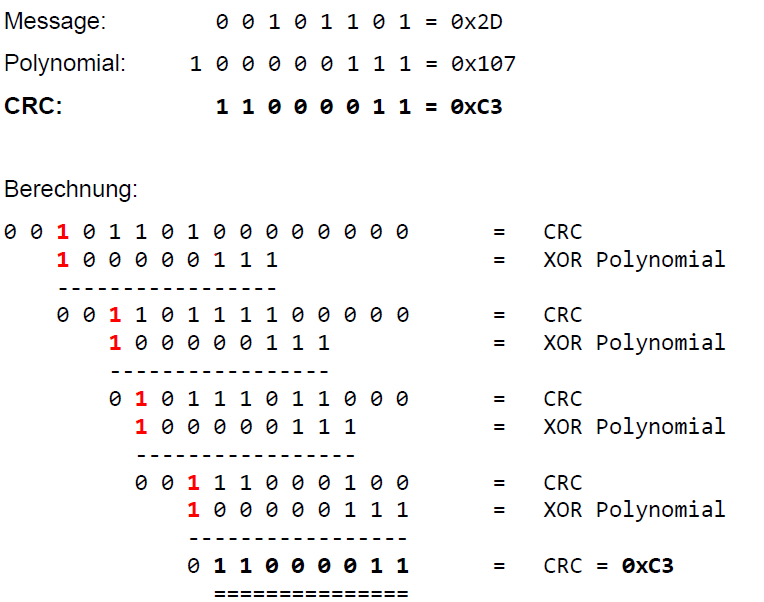
\includegraphics[width=.6\linewidth]{900-Praktika/prak06/crc1.PNG}
\end{center}

\subsection{Aufgabe 2: Verifikation empfangener Daten mittels CRC}

Nach einer seriellen Übertragung wurden die folgenden drei Messages empfangen. Dabei entspricht das erste
Byte den \textcolor{blue}{Daten} und das zweite der \textcolor{orange}{CRC-Prüfsumme} (MSB first). Das verwendete Generatorpolynom ist
dasselbe wie in Aufgabe 1 (CRC-8 CCITT).

Überprüfen Sie, welche der drei Messages fehlerfrei übertragen wurden und welche nicht.

\subsubsection{Lösung}
\begin{center}
  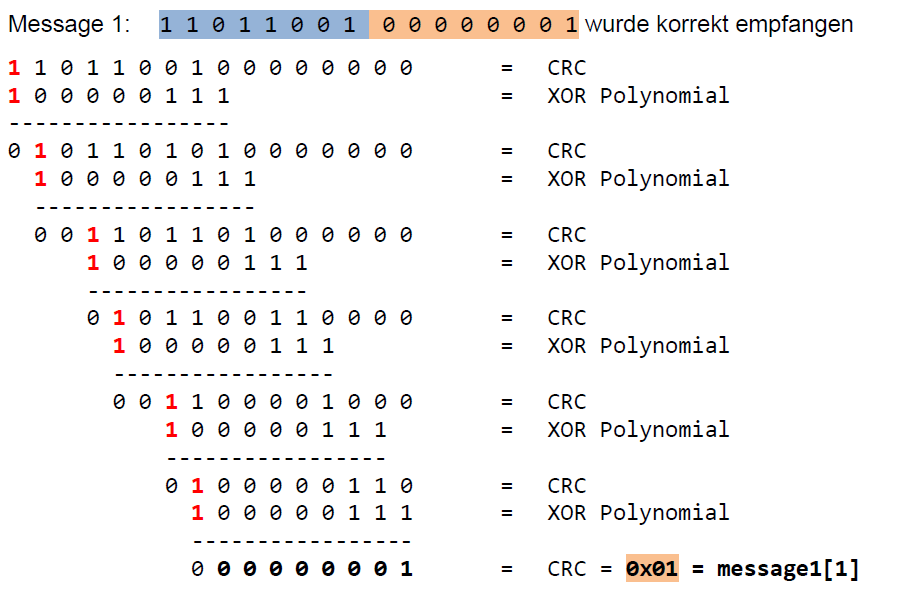
\includegraphics[width=.6\linewidth]{900-Praktika/prak06/crc2.PNG}
\end{center}

Bei der noch einfacheren Möglichkeit zur Verifikation werden die gesamten empfangenen Daten inklusive der Prüfbits durch das Generatorpolynom gelassen. Wenn alles korrekt ist, so muss am Schluss der Wert 0 als CRC übrigbleiben

\begin{center}
  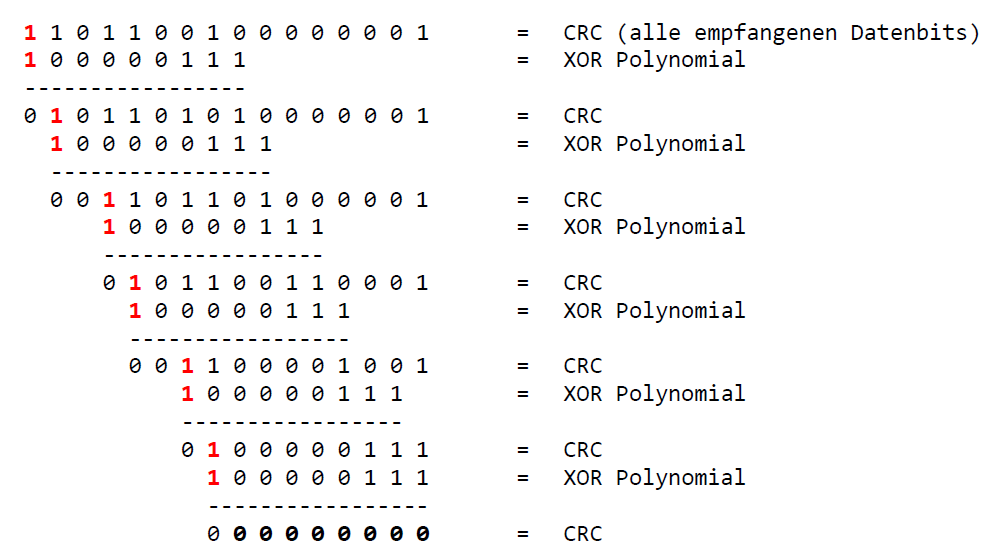
\includegraphics[width=.6\linewidth]{900-Praktika/prak06/crc3.PNG}
  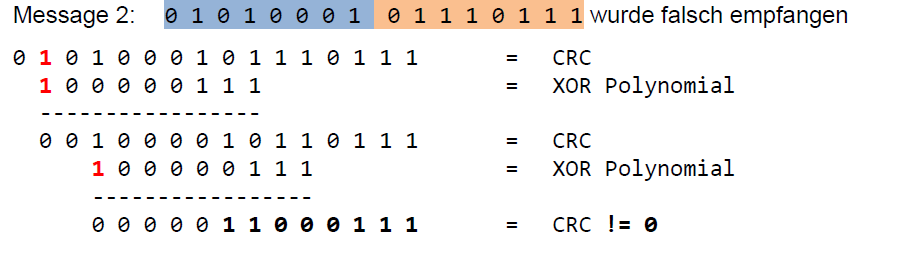
\includegraphics[width=.6\linewidth]{900-Praktika/prak06/crc4.PNG}
\end{center}

Die zweite Message wurde falsch empfangen. Entweder ist das Daten- oder das Prüfsummenbyte korrupt. Der Empfänger muss in einem solchen Fall ein NAK zurückgeben, um die Message noch einmal anzufordern.

\subsection{Aufgabe 3: C++ - Implementation}
Implementieren Sie eine Klasse Crc, welche die Prüfsumme CRC-8 CCITT mit Schiebeoperationen auf Bit-
Ebene berechnet. Um den Algorithmus zu überprüfen, soll ein Testprogramm geschrieben werden, welches
entweder die Prüfsumme der Datenbytes aus Aufgabe 2 berechnet, oder die Prüfsumme der vorgegebenen
Datei ausgibt. Der Dateiname soll der Applikation als Argument übergeben werden.

\subsubsection{Lösung}

Wird das Programm ohne Argument aufgerufen, berechnet es die Prüfsumme von {0xd9, 0x51, 0x61}.

\begin{lstlisting}[language=C++, style=C++]
$ ./crcTest
CRC-8 CCITT Bit um Bit, einfach aber ineffizient

CRC-8 CCITT der einzelnen Datenbytes:
Byte 00: crc(0xd9) = 0x01
Byte 01: crc(0x51) = 0xb0
Byte 02: crc(0x61) = 0x20
CRC-8 CCITT von allen Datenbytes:
crc(0xd95161) = 0x2c
\end{lstlisting}

Mit einem gültigen Dateinamen als Argument wird diese Datei in einen Byte-Buffer gelesen und die Prüfsum-me über den gesamten Buffer berechnet.

\begin{lstlisting}[language=C++, style=C++]
$ ./crcTest datafile.txt
CRC-8 CCITT Bit um Bit, einfach aber ineffizient
Datei: datafile.txt
Anzahl Datenbytes: 72125
CRC-8 CCITT: 0x10
\end{lstlisting}

\lstinputlisting[language=C++, style=C++, multicols=2]{900-Praktika/prak06/Loesung/A3/Crc.h}
\noindent\makebox[\linewidth]{\rule{\paperwidth}{0.4pt}}
\lstinputlisting[language=C++, style=C++, multicols=2]{900-Praktika/prak06/Loesung/A3/Crc.cpp}
\noindent\makebox[\linewidth]{\rule{\paperwidth}{0.4pt}}
\lstinputlisting[language=C++, style=C++, multicols=2]{900-Praktika/prak06/Loesung/A3/CrcTest.cpp}

\subsection{Aufgabe 4: C++ - Implementation mit einer Lookup Tabelle}
Implementieren Sie eine Klasse Crc, welche die Prüfsumme CRC-8 CCITT mit Hilfe einer 8 Bit breiten Lookup
Tabelle berechnet. Die Lookup Tabelle kann im Voraus berechnet werden oder sogar konstant im ROM
abgelegt werden.
Um den Algorithmus zu überprüfen soll ein Testprogramm geschrieben werden, welches entweder die Prüfsumme
der Datenbytes aus Aufgabe 2 berechnet, oder die Prüfsumme der vorgegebenen Datei ausgibt. Der
Dateiname soll der Applikation als Argument übergeben werden. Variieren Sie die Dateigrösse und vergleichen
Sie die Berechnungszeit mit der Variante aus der Aufgabe 3.

\medskip

Hinweis File I/=:

\begin{lstlisting}[language=C++, style=C++]
#include <fstream>
 ...
f.open(argv[1], ios::in | ios::binary);
// determine file size
f.seekg(0, ios::end);
len = f.tellg();
f.seekg(0, ios::beg);
// Allocate byte buffer
buf = new uint8_t[len];
// read file content into byte buffer
f.read((char*)buf, len);
f.close();
// ...
delete[] buf; // free allocated memory
\end{lstlisting}

\subsubsection{Lösung}


\lstinputlisting[language=C++, style=C++, multicols=2]{900-Praktika/prak06/Loesung/A4/Crc.h}
\noindent\makebox[\linewidth]{\rule{\paperwidth}{0.4pt}}
\lstinputlisting[language=C++, style=C++, multicols=2]{900-Praktika/prak06/Loesung/A4/Crc.cpp}
\noindent\makebox[\linewidth]{\rule{\paperwidth}{0.4pt}}
\lstinputlisting[language=C++, style=C++, multicols=2]{900-Praktika/prak06/Loesung/A4/CrcTest.cpp}

\subsection{Aufgabe 5: C++ - Implementation mit einer Lookup Tabelle}

Mit dem Tool Callgrind kann die Laufzeit eines Programms analysiert werden. In der Standardkonfiguration
werden die Anzahl der ausgeführten Instruktionen aufgezeichnet. Die aufgezeichnete Anzahl der Instruktionen
wird zudem mit Sourcecode-Zeilen und Funktionsaufrufen in Beziehung gesetzt. Zusätzlich kann eine
Cachesimulation aktiviert werden, die weitere Informationen über die Laufzeitperformance des Programms
geben kann. Die Cachesimulation führt das gleiche aus wie das Tool Cachegrind. Callgrind schreibt das Ergebnis
der Laufzeitanalyse in eine Datei. Die Datei kann dann mit dem Programm KCachegrind visualisiert
werden.

\url{http://valgrind.org/docs/manual/cl-manual.html}
\url{http://valgrind.org/docs/manual/cg-manual.html}

In dieser Aufgabe sollen Sie die CRC-8 CCITT Implementationen mittels Tabelle und mittels Schiebeoperationen
auf Bit-Ebene mit Valgrind profilen.

Beachten Sie die Vorgabe und binden Sie Ihre eigenen CRC-Implementationen ein.

Callgrind: Profilen Sie die beiden CRC Implementationen mit dem Tool Callgrind. Visualisieren sie die Ausgabe
mit KCachegrind und untersuchen sie die Performanceunterschiede.
\begin{enumerate}
  \item In welchem Sourcecode-File liegt der Hotspot. Auf welchen Sourcecode-Zeilen liegt der Hotspot im
  entsprechenden File für die CRC-Berechnung? Wie unterscheiden sich die beiden Implementationen
  bezüglich Laufzeitperformance?
  \item Wie verändert sich die Performance der beiden Programme, wenn mit Optimierungsstufe –O3 kompiliert
  wird? Verändert sich der Hotspot der beiden CRC-8 Implementationen gleichermassen mit eingeschalteter
  Optimierung?
\end{enumerate}

\textbf{Hinweis:} Übergeben Sie für das Callgrind-Profiling das datafile.txt dem CRC Testprogramm, damit der
CRC über einige Bytes berechnet werden muss und dadurch der Overhead für Systemfunktionen bezogen
auf die CRC Berechnung kleiner wird.

\subsubsection{Lösung}

Die verwendeten Profiling-Befehle finden Sie in den make-Files in ./Loesung/A5.

\begin{enumerate}
  \item Bei beiden Implementationen benötigt die Funktion \texttt{Crc::getCrc()} aus crc.cpp am meisten Rechenzeit. In dieser Funktion liegt der Hotspot bei der for-Schleife. Der Unterschied der beiden Implementationen kann an der Anzahl Zyklen festgestellt werden. Bei der Tabellenimplementation werden 1‘442‘513 Zyklen und bei der Schiebeoperationsvariante 7‘571‘101 Zyklen verbraucht. Daraus geht hervor, dass die Tabellenvariante etwa 5.2-mal schneller ist als die Schiebeoperationsvariante.

  \lstinputlisting[language=C++, style=C++, multicols=2]{900-Praktika/prak06/Loesung/A5/CrcBitWise/makefile}
  \noindent\makebox[\linewidth]{\rule{\paperwidth}{0.4pt}}
\lstinputlisting[language=C++, style=C++, multicols=2]{900-Praktika/prak06/Loesung/A5/CrcBitWiseO3/makefile}

  \item Die Schiebeoperationsvariante reduziert die Anzahl der Zyklen um 70 \% auf 2‘235‘591 Zyklen und die Tabellenvariante ebenfalls um 70 \% auf 432‘757 Zyklen.

  \lstinputlisting[language=C++, style=C++, multicols=2]{900-Praktika/prak06/Loesung/A5/CrcWithTable/makefile}
  \noindent\makebox[\linewidth]{\rule{\paperwidth}{0.4pt}}
\lstinputlisting[language=C++, style=C++, multicols=2]{900-Praktika/prak06/Loesung/A5/CrcWithTableO3/makefile}
\end{enumerate}
